\documentclass[a4paper, 12pt]{extarticle}

%% подключаем стандарт библиографии
\bibliographystyle{gost71u}

%% для "Abstract" в классе book
% \newenvironment{abstract}{}{}
% \usepackage{abstract}

%% подключаем преамбулу: в ней содержится подключение всех необходимых пакетов
%% Работа с русским языком
\usepackage{cmap}			 % поиск в PDF
\usepackage{mathtext} 		 % русские буквы в формулах
\usepackage[T2A]{fontenc}	 % кодировка
\usepackage[utf8]{inputenc}	 % кодировка исходного текста
\usepackage[russian, english]{babel}	 % локализация и переносы

%% Пакеты для работы с математикой
\usepackage{amsmath,amsfonts,amssymb,amsthm,mathtools}
\usepackage{icomma}

%% Нумерация формул (опционально)
%\mathtoolsset{showonlyrefs=true} % показывать номера только у тех формул, на которые есть \eqref{} в тексте.
%\usepackage{leqno}               % нумерация формул слева

%% Шрифты
\usepackage{euscript}	 % шрифт "Евклид"
\usepackage{mathrsfs}    % красивый мат. шрифт

%% Некоторые полезные макросы для дебага (в случае недоверия авторам шаблона)
\makeatletter
\newcommand\thefontsize{The current font size is: \f@size pt} % пример: \section{\thefontsize}
\makeatother
\usepackage{xcolor}

%% Настройка размеров шрифтов
\makeatletter
\setlength{\headheight}{28pt}

\usepackage{geometry} % Меняем поля страницы
\geometry{left=3cm}% левое поле
\geometry{right=2cm}% правое поле
\geometry{top=2cm}% верхнее поле
\geometry{bottom=2cm}% нижнее поле

\def\theequation{\thesection.\arabic{equation}}

\renewcommand{\baselinestretch}{1.5}
\renewcommand{\vec}{\mathbf}
\DeclareMathOperator{\erf}{erf}

%% Русские списки
\usepackage{enumitem}
\makeatletter
\AddEnumerateCounter{\asbuk}{\russian@alph}{щ}
\makeatother

%% Работа с картинками
\usepackage{caption} % пакет для подписей к рисункам, в частности, для работы caption*
\captionsetup{justification=centering} % центрирование подписей к картинкам
\usepackage{graphicx}                  % вставки рисунков
\graphicspath{{images/}{images2/}}     % папки с картинками
\setlength\fboxsep{3pt}                % отступ рамки \fbox{} от рисунка
\setlength\fboxrule{1pt}               % толщина линий рамки \fbox{}
\usepackage{wrapfig}                   % обтекание рисунков и таблиц текстом

%% Работа с таблицами
\usepackage{array,tabularx,tabulary,booktabs} % дополнительная работа с таблицами
\usepackage{longtable}                        % длинные таблицы
\usepackage{multirow}                         % слияние строк и столбцов в таблице
\usepackage{makecell}                         % создание ячеек с многими строчками текста
\usepackage{hhline}                           % позволяет разрывать горизонтальные линии в таблицах

%% Перенос знаков в формулах (по Львовскому)
\newcommand*{\hm}[1]{#1\nobreak\discretionary{}{\hbox{$\mathsurround=0pt #1$}}{}}

% Hyperref (для ссылок внутри  pdf)
\usepackage[unicode, pdftex]{hyperref}

% Отступ перед первым абзацем в каждом разделе
\usepackage{indentfirst}


\begin{document}
	
    %% титульник
    \begin{center}
    	%% *название института*
    	\large\textbf{Министерство науки и высшего образования Российской Федерации\\
    		Московский физико-технический институт (государственный
    		университет)} \\
    	\vspace{1cm}
    	
    	%% *факультет/физтех-школа*
    	Физтех-школа физики и исследований им. Ландау \\
    	
    	%% *название базовой кафедры и лаборатории*
    	%% в случае ненадобности можно удалить
    	Кафедра вычислительной физики конденсированного состояния и живых систем \\
    	Лаборатория №1.6 теплофизических баз данных ОИВТ РАН\\
    	
    	\vspace{3em}
    	
    	Выпускная квалификационная работа бакалавра
    \end{center}
    
    \begin{center}
    	\vspace{\fill}
    	%% *название вашей работы*
    	\LARGE{Квантово-механические расчеты и термодинамические функции карбидов аргона}
    	
    	\vspace{\fill}
    \end{center}
    
    
    \begin{flushright}
    	\textbf{Автор:} \\
    	Студент 203 группы\\
    	Щерба Александр Андреевич \\
    	\vspace{2em}
    	\textbf{Научный руководитель:} \\
    	Доктор физико-математических наук \\
    	Мальцев Максим Александрович \\
    \end{flushright}
    
    \vspace{7em}
    
    \begin{center}
    	%% *лого*
    	
\includegraphics[width=100 pt]{MIPT_logo.jpg}\\
    	Москва \the\year{}
    \end{center}
    
    %% выключаем отображение номера для этой страницы (титульник)
    \thispagestyle{empty}
    
    \newpage

    %% аннотация
    \begin{abstract}
    	
    	\begin{center}
    		\large{Квантово-механические расчеты и термодинамические функции карбидов аргона} \\
    		\large\textit{Иванов Иван Иванович} \\[1 cm]
    		
    		Были вычислены межатомные потенциалы для 21 низколежащего состояния иона ArC$^+$, охватывающие оба предела диссоциации Ar($^1$S) -- C$^+$($^2$ P) и Ar$^+$($^2$P) -- C($^3$P). Расчеты были выполнены на уровне теории CASSCF/MRACPF2a с использованием базисных наборов aug-cc-pwCVnZ (n=T, Q) с последующей экстраполяцией к пределу CBS. На основе численно рассчитанных энергетических спектров были оценены зависящие от температуры термодинамические функции в диапазоне 298.15 -- 20000 K. Также было оценено влияние включения возбужденных электронных состояний в термодинамические расчеты.
    		
    		СТАТЬЯ
		    
    		    
    		\vfill
    		
    		\textbf{Abstract} \\[1 cm]
    	\end{center}
    	
    \end{abstract}
    \newpage

    %% содержание
    \tableofcontents{}
    \newpage

    % \fontsize{14}{16}\selectfont
    \section{Введение}
    
    \subsection{Актуальность работы}
    \label{sec:Chapter0.1}
    
    \subsection{Постановка задачи}
    \label{sec:Chapter0.2}
    
    \subsection{Обзор литературы}
    \label{sec:Chapter0.3}
    
    \newpage
    \section{Методы квантово-механического расчета}
   
    \subsection{Теоретические основы квантово-химических расчетов}
    \label{sec:Chapter1.1}
    
    Квантовая химия -- раздел теоретической химии, в котором методами квантовой механики исследуется электронная структура молекулярной системы, информация о которой используется для определения структурных, химических и энергетических свойств. Задачей методов квантовой химии ставиться нахождение волновой функции собственной к фиксированному гамильтониану системы, определяемой в стационарном уравнении Шредингера \ref{eq:schrodinger}. Этот гамильтониан можно разбить набор энергетических операторов, отвечающих отдельным элементам движения и взаимодействия в системе. В случае присутствия $K$ атомов и $N$ электронов мы также вводим координатное представление волновой функции, в котором появляется зависимость от  координат атомов $\boldsymbol{R} = (\vec{R_1},\ ...\ , \vec{R_K})$, а также координат и спинов электронов $\boldsymbol{r} = (\vec{r_1},\ ...\ , \vec{r_N})$, $\boldsymbol{\sigma} = (\sigma_1,\ ...\ , \sigma_N)$.
    
    \begin{equation} \label{eq:schrodinger}
		\begin{split}
			&\hat{H} \psi = E \psi, \quad \psi = \psi(\boldsymbol{R}, \boldsymbol{r}, \boldsymbol{\sigma} ) \\
			&\hat{T}+\hat{V}=\hat{T}_\text{n}+\hat{T}_\text{e}+\hat{V}_\text{ne}+\hat{V}_\text{ee}+\hat{V}_\text{nn}
		\end{split}
    \end{equation}
    
    Для систем, включающих в себя большое количество электронов, аналитическое определение волновой функции становится невозможным. Альтернативным способом расчета являются численные методы, основанные на нескольких базовых приближениях и позволяющие получать волновую функцию с точностью, достаточной для корректного определения интересующих нас свойств системы.
    
    Первым является приближение Борна-Оппенгеймера \cite{born-opper}, заключающиеся в разделении движения легких электронов и тяжелых ядер. Рассматривая систему, как единую движущуюся в пространстве конструкцию, можно сделать предположение о схожести порядков импульсов между электронами и ядрами. В то же время их массы отличаются минимум на три порядка, что дает основание рассматривать ядра неподвижными относительно электронов. Это выражается в выделении из полного гамильтониана электронной части и формирования соответствующего уравнения Шредингера \ref{eq:born-opper}, называемого электронным. Здесь набор координат атомов $\boldsymbol{R}$ становится фиксированным параметром, варьируя который можно находить электронную структуры системы в различных положениях атомного остова. Получаемая при этом зависимость $E(\boldsymbol{R})$ называется поверхностью потенциальной энергии (ППЭ).
    
    \begin{equation} \label{eq:born-opper}
    	\begin{split}
    		&\hat{H}_\text{e} \psi_\text{e}(\boldsymbol{r}, \boldsymbol{\sigma} \mid \boldsymbol{R})=E_\text{e}(\boldsymbol{R}) \psi_\text{e}(\boldsymbol{r}, \boldsymbol{\sigma} \mid \boldsymbol{R}) \\
    		&\hat{H} = \hat{T}_\text{e}+\hat{V}_\text{ne}+\hat{V}_\text{ee}+\hat{V}_\text{nn}
    	\end{split}
    \end{equation}
    
    Таким образом задача сводиться к расчету многоэлектронной волновой функции $\psi_e$ (далее для краткости называемой электронной). Связь с полной волновой функцией $\psi$ системы состоит в использовании полученных $\psi_e$ в качестве ортонормированного базиса \ref{eq:atomic}, где коэффициенты линейного разложения $\chi_k(\boldsymbol{R})$ получаются из уравнения ниже. Здесь энергия $E$ соответствует уже полной энергии системы и не зависит от $\boldsymbol{R}$, то есть отражает уровни энергии системы, используемые при расчете статистической суммы.
    
    \begin{equation} \label{eq:atomic}
    	\begin{split}
    		&\psi=\sum_{k=0}^{\infty} \chi_k(\boldsymbol{R}) \psi_{\text{e}, k}(\boldsymbol{r} \mid \boldsymbol{R}) \\
    		&\left[\hat{T}_n+E_m(\boldsymbol{R})\right] \chi_m+\langle \psi_{\text{e}, m} | \hat{T}_n | \psi_{\text{e}, m} \rangle \chi_m=E \chi_m
    	\end{split}
    \end{equation}
    
    
    Возвращаясь к электронному уравнению Шредингера, при раскрытии энергетических операторов мы получаем систему дифференциальных уравнений, решение которой возможно методом рядов Фурье. Выбор базиса для разложения электронной волновой функции $\psi_\text{e}$ является предметом второго приближения.
    
    В начале вводится набор функций молекулярных спин-орбиталей (МО) $\{\phi_i (\vec{r_j}, \sigma_j)  \}_{i=1}^{i=M}$, где каждая отражает некую i-ю возможную область пространства, занимаемую j-м электроном. Для гибкости их определяют через линейные комбинации фиксированного набора атомных орбиталей $\chi_{\text{e},k}$ с варьируемыми коэффициентами $c_k$ (здесь $\chi_{\text{e},k}$ обычно задается комбинацией гауссиан). Выбрав из $M$ спин-орбиталей $N$ занятых электронами, мы можем построить набор всевозможных конфигурационных функций состояний $\{\Phi_I \}$. Так как здесь $\Phi_I$ представляет собой некоторую конфигурацию системы (фиксированное распределение электронов по молекулярным орбиталям), то можно искать итоговую электронную волновую функцию в пространстве всех таких конфигураций \ref{eq:slater}. Для соблюдения принципа Паули, а также правильной спиновой и пространственной симметрии удобно строить $\Phi_I$ через линейные комбинации детерминантов Слейтера.
    
    \begin{equation} \label{eq:slater}
    \psi_\text{e} = \sum_{k=1}^L C_I \Phi_I, \quad \Phi_I=\frac{1}{\sqrt{N!}} \sum_{K=\sigma\left(k_1, \ldots, k_N\right)}(-1)^p \phi_{k_1}(1) \ldots \phi_{k_N}(N)
	\end{equation}
      	
    Таким образом нахождение электронной волновой функции $\psi_\text{e}$ в методах квантовой химии сводится к численному нахождению коэффициентов $c_k$ и $C_I$, определяющих $\psi_\text{e}$ как собственную волновую функцию электронного гамильтониана $\hat{H}_\text{e}$. Оба набора коэффициентов разложения подбираются вариационным методом, основанном на минимизации энергии системы. Для дальнейшего анализа полное пространство полученных молекулярных орбиталей целесообразно разделить на три непересекающиеся группы в соответствии с их характером заселенности:
    \begin{enumerate}
    	\item остовные (core) - орбитали внутренних электронных оболочек, которые остаются дважды занятыми во всех конфигурациях;
    	\item виртуальные (virtual) - свободные орбитали, заселенность которых в исходном пространстве равна нулю;
    	\item активные (active) - орбитали, заселенность которых варьируется от 0 до 2 как в рамках многоконфигурационного разложения, так и при изменении межъядерного расстояния R.
    \end{enumerate}
  
  	Основным отличием методов квантовой химии является размерность пространства конфигурационных функций состояний $\{\Phi_I \}$, над которым строится электронная волновая функция $\psi_\text{e}$. Приближения, используемые различными методами для уменьшения этой размерности влияет на точность и их вычислительную сложность. В данной работе для расчета ППЭ соединений ArC и ArC$^+$ используется сочетание методов самосогласованного поля в полном активном пространстве и многоконфигурационного взаимодействия, являющихся более вычислительно затратными. Такое решение продиктовано сложностью орбитальной структуры исследуемых молекул и сильным влиянием электронной корреляции. Правильный учет последней играет критическую роль в корректном определении глубины энергетических ям для связанных состояний обоих карбидов.
    
    \subsection{Метод самосогласованного поля в полном активном пространстве}
    \label{sec:Chapter1.2}
    
    Одним из активно используемых в работе алгоритмов квантовой химии является метод самосогласованного поля в полном активном пространстве (complete active space self consistent field, CASSCF), он затрагивает первый из двух видов электронной корреляции - статический. Основная проблема статической корреляции заключается в правильном определении энергии состояния с несколькими ведущими конфигурационными функциями $\Phi_I$. Ввиду того, что алгоритмы Хартри-Фока, теории возмущений и связанных кластеров исходят из предположения о единственной ведущей $\Phi_0$ (берется минимальная размерность пространства $\{ \Phi_I \}$), точный расчет энергии упомянутых состояний этими методами не представляется возможным. В то же время CASSCF является одним из наименее вычислительно затратных методов, решающих данную проблему.
    
    Для этого электронная волновая функция $\psi_e$ рассчитывается в пространстве подпространстве конфигурационных функций $\{ \Phi_I \}^\text{act}$, порождаемое всевозможными перестановками внутри активного пространства. Такое ограниченное расширение позволяет одновременно избежать проклятия размерности (экспоненциального увеличения возможных $\Phi_I$ при рассмотрении большего числа молекулярных орбиталей) и при этом получить наиболее важные результаты многодетерминантного подхода.
    
    Помимо учета статической корреляции таким важным результатом также является возможность оптимизации энергии для нескольких состояний системы, ввиду возможности $\{ \Phi_I \}^\text{act}$ одновременно включать в себя ведущие функции нескольких состояний. Еще одним преимуществом является подбор молекулярных орбиталей $c_k$ с учетом нескольких состояний в алгоритме самосогласованного поля, что также является выделяющейся чертой метода CASSCF. Определив теоретическую базу многоконфигурационного подхода, перейдем к описанию конкретных вычислительных параметров расчета CASSCF, использованных в настоящей работе.
    
     Для обоих молекул при оптимизации орбиталей CASSCF глубоколежащие C(1s), Ar(1s), Ar(2s) и Ar(2p) были заморожены, тогда как занятые орбитали C(2s), C(2p) и Ar(3p) были выбраны в качестве активных орбиталей. Полученное пространство молекулярных орбиталей обозначается как случай CAS(9,7), каждая MO маркируется согласно атомной орбитали с наибольшим процентным вкладом на пределе диссоциации. Отдельно для ArC в пространство активных орбиталей была дополнительно включена C(3s).
    
    Также в рамках расчетов ионизированного карбида аргона возникает трудность из-за различных ионизированных атомов в двух пределах диссоциации, что приводит к различной диффузности связанных с каждым пределом молекулярных орбиталей. Эта проблема проявляется через появление вкладов более и менее диффузных атомных орбиталей в составах активных MO. Таким образом, выбранные орбитали должны одновременно описывать две различные физические ситуации, дополнительно усиливая проблему "компромиссных орбиталей". Для иллюстрации этой проблемы ниже показан нормированный состав орбитали C(2p) в системе ArC$^+$ при 6.4 \AA\ для различных схем усреднения по состояниям:
    
    \begin{enumerate}
    	\item Включение состояний, отвечающих пределу диссоциации Ar -- C$^+$: C(2p) $\sim$ 0.58 C(1p), 0.78 C(2p), 0.23 C(3p)
    	\item Включение состояний, отвечающих пределу диссоциации Ar$^+$ -- C: C(2p) $\sim$ 0.51 C(1p), 0.73 C(2p), 0.45 C(3p)
    \end{enumerate}
    
    Для решения данной проблемы применялась процедура усреднения по состояниям (state averaged CASSCF, SA-CASSCF) со специальной схемой задания весовых коэффициентов, обеспечивающей равноправный вклад каждого асимптотического предела. Суммарные веса двух пределов были выбраны равными, при этом веса состояний внутри каждого предела распределялись равномерно. Корректность использованных весов проверялась путем сопоставления рассчитанных чисел заселенности молекулярных орбиталей (МО) с значениями заселенностей, полученных путем усреднения конфигураций различных пределов диссоциации между собой.
    
    В случае обоих молекул активное пространство выбиралось с учетом основных и возбужденных состояний, которые необходимо рассмотреть. Выбранная стратегия позволила получить молекулярные орбитали, в равной степени хорошо описывающие все состояния. Вычисленный методом SA-CASSCF набор конфигурационных функций состояний также является хорошим приближением, но не учитывает более высокоэнергичные конфигурации молекул. Для дальнейшего уточнения результатов над построенным SA-CASSCF пространтвом молекулярных орбиталей проводится расчет методом MRACPF2a.
    
    
    \subsection{Многорференсный метод конфигурационного взаимодействия}
    \label{sec:Chapter1.3}
    
    Следующий метод позволяет учесть влияние динамической корреляции на точность результатов. Данный эффект отражает кулоновское отталкивание электронов при их взаимном сближении, что приводит к появлению локального минимума амплитуды волновой функции вблизи нулевого межэлектронного расстояния. Для описания данного эффекта приходиться вводить большое число возбужденных конфигураций, которые с одной стороны позволяют учесть столкновения электронов через их возбуждение, а с другой расширяют пространство $\{ \Phi_I \}$ в достаточной мере для правильной аппроксимации волновой функции в области малого межэлектронного расстояния.
    
    Соответствующий учету данного эффекта метод называется конфигурационным взаимодействием (configuration interaction, CI). Включение в расчет всевозможных возбужденных конфигурационных функций состояния влечет экспоненциальный рост вычислительных затрат, полученная такая таким образом волновая функция считается точной (над отдельно выделенным пространством молекулярных орбиталей), а соответствующий метод FullCI является эталонным. Однако для сохранения разумного времени расчета с получением достаточной точности обычно ограничиваются одно- и двух- кратными возбуждениями ограниченного набора $\{ \Phi_I \}^\text{act}$, определяемыми в CASSCF. Упрощенная подобным образом схема является вариантом многореференсного метода конфигурационного взаимодействия (multireference configuration interaction, MRCI(SD)).
    
    В данной работе используется дополненный к MRCISD метод, модифицированный специально для соблюдения размерной экстенсивности. Проблема состоит в несоответствии полной энергии системы на пределе диссоциации и суммы энергий ее отдельных частей, а причиной служит отсутствие учета более высоких возбуждений. В модифицированной версии для включения данного эффекта вводится измененная нормировка функционала энергии \ref{eq:acpf}.После разделения волновой функции на рефернсную и корреляционную части ($\psi = \psi_0 + \psi_c$, $\langle \psi_0 \mid \psi_c \rangle = 0$) последняя дополнительно делится на элемент внутренних возбуждений активного простанства $\psi_a$ и оставшихся $\psi_l$. В отличии от метода MRCI имеющего коэффициенты нормировки $g_a = g_l = 1$, модифицированный метод определяет $g_c = \frac{2}{n}$. Построенный таким образом нормировочный знаменатель позволяет эффективно учесть эффекты несвязанных кластеров (unlinked-cluster effects). Полученная схема называется мультирефернсым методом усредненного функционала связанных пар (Averaged Coupled-Pair Functional, MRACPF) \cite{gdanitz_acpf}.
    
    \begin{equation} \label{eq:acpf}
	    E_c\left[\Psi_c\right]:=\frac{\left\langle\Psi_0+\Psi_c\right| \hat{H}-E_0\left|\Psi_0+\Psi_c\right\rangle}{1+g_a\left\langle\Psi_a \mid \Psi_a\right\rangle+g_e\left\langle\Psi_e \mid \Psi_e\right\rangle}
    \end{equation}
    
    Итоговая схема расчета ППЭ для молекул ArC и ArC$^+$ включает в себя получение пространства молекулярных орбиталей и референсных конфигурационных функций методом SA-CASSCF, на основе которых проводится учет динамической корреляции численно улучшенным методом MRACPF2a.
    
    
    \subsection{Пакет Orca и получаемые результаты}
    \label{sec:Chapter1.4}
     
    Практическая реализация вышеописанных квантово-химических методов и расчет потенциальных кривых исследуемой системы выполнялись с использованием современного программного комплекса Orca 6.1.0-f.0 \cite{neese_orca}. Данный пакет оптимизирован для проведения высокоуровневых многоконфигурационных расчетов SA-CASSCF и MRACPF2a. Вместе с тем, для анализа полученных результатов (извлечение, обработка и визуализация массивов данных квантово-химического вывода) был разработан собственный программный скрипт на языке Python. При написании также использовался пакет Orca Python Interpeter \cite{opi}, созданный той же командой для удобного управления расчетом и обработки данных.
    
    Реализации методов CASSCF и MRACPF2a, доступные в пакете Orca \cite{neese_orca}, использовались совместно с расширенными корреляционно-согласованными базисными наборами aug-cc-pwCVnZ (n=T, Q). Все результаты были экстраполированы к пределу полного базисного набора aug-cc-pwCV$\infty$Z (CBS). Для использования пространственной симметрии в расчетах симметрия $C_{\infty v}$ линейных соединений ArC и ArC$^+$ была сопоставлена с ее абелевой подгруппой $C_{2 v}$. Такое представление дает неприводимые представления $A_1$, $A_2$ и пару $B_1 / B_2$. Эти представления служат метками симметрии, которые классифицируют электронные волновые функции согласно их отклику на операции редуцированной группы симметрии. При корреляции $C_{\infty v} \to C_{2 v}$ состояния $\Sigma^+$ и $\Sigma^-$ соответствуют $A_1$ и $A_2$ соответственно, тогда как состояния $\Pi$ коррелируют с парой $B_1/B_2$, а состояния $\Delta$ — с парой $A_1/A_2$.
    
    Расчеты для ArC$^+$ были выполнены на радиальной сетке, состоящей из 60 точек от 1.4 до 4.4 \AA\ и 10 дополнительных точек от 4.4 до 6.4 \AA. Итоговый набор состояний, разделенных по неприводимым представлениям, выглядит следующим образом; здесь целое число перед меткой неприводимого представления обозначает число состояний этой симметрии, включенных в расчет:
    
    \begin{enumerate}
    	\item Ar($3s^23p^6$; $^1$S) -- C$^+$($2s^22p^1$; $^2$ P): $1A_1$, $1B_1$, $1B_2$ для дублета
    	\item Ar$^+$($3s^23p^5$; $^2$P) -- C($2s^22p^2$; $^3$P): $2A_1$, $3A_2$, $2B_1$, $2B_2$ для дублета и квартета
    \end{enumerate}
    
   	Аналогичные вычисления были проделаны для нейтральной молекулы ArC. Ввиду крайне слабой связанности этого соединения включение высоко возбужденных состояний является необходимым условием правильного определения термодинамических функций. В рамках SA-CASSCF/MRACPF2a расчета на сетке межъядерных расстояний, включающей 60 точек в диапазоне 1.4--3.4 \AA\ и 8 точки в интервале 3.4--4.4 \AA, было получено 18 состояний различных пределов диссоциации:
   	
    \begin{enumerate}
    	\item $\text{Ar}\left({ }^1 S_g\right)\text{ -- }\text{C}\left({ }^3 P_g ; 2 s^2 2 p^2\right)$: $1A_2$, $1B_1$, $1B_2$ для триплета
    	\item $\operatorname{Ar}\left({ }^1 S_g\right) \text{ -- }\text{C}\left({ }^1 D_g ; 2 s^2 2 p^2\right)$: $2A_1$, $1A_2$, $1B_1$, $1B_2$ для синглета
    	\item $\operatorname{Ar}\left({ }^1 S_g\right) \text{ -- } \text{C}\left({ }^1 S_g ; 2 s^2 2 p^2\right)$: $1A_1$ для синглета
    	\item $\operatorname{Ar}\left({ }^1 S_g\right) \text{ -- } \text{C}\left({ }^5 S_u ; 2 s^1 2 p^3\right)$: $1A_2$ для квинтета
    	\item $\operatorname{Ar}\left({ }^1 S_g\right) \text{ -- } \text{C}\left({ }^3 P_u ; 2 s^2 2 p^1 3 s^1\right)$: $1A_1$, $1B_1$, $1B_2$ для триплета
    	\item $\operatorname{Ar}\left({ }^1 S_g\right) \text{ -- } \text{C}\left({ }^3 D_u ; 2 s^2 2 p^1 3 d^1\right)$: $1A_1$, $2A_2$, $1B_1$, $1B_2$ для триплета
    \end{enumerate}
    
    Порядковый номер электронного состояния конкретной мультиплетности и пространственной симметрии (терма) будем обозначать цифрой в скобках, указываемой перед его символом. Несмотря на то, что лишь некоторые из этих состояний имеют потенциальные ямы, критически важные для последующего расчета термодинамических функций, включение всего набора состояний в процедуру усреднения необходимо. Такой подход позволяет предотвратить искусственное нарушение пространственной симметрии волновой функции и обеспечить корректные (физически оправданные) числа заселенности молекулярных орбиталей в активном пространстве
    
    Все расчеты выполнялись в режиме сканирования поверхности потенциальной энергии в направлении уменьшения межъядерного расстояния. Молекулярные орбитали из ранее рассчитанной точки повторно использовались в качестве начального приближения. Такой подход позволяет избежать перестановки молекулярных орбиталей внутри активного пространства и упрощает использование данных неприводимых представлений для построения пространства активных орбиталей. Результаты, полученные с использованием базисных наборов aug-cc-pwCVnZ (n=T,Q), были поточечно экстраполированы к пределу CBS с использованием формулы Хельгакера ($\sim n^{-3}$)~\cite{helgaker_cbs}.

    \newpage
    \section{Расчет термодинамических функций}
    
    \subsection{Энергетический спектр состояний}
    \label{sec:Chapter2.1}

	Расчет термодинамических функций проводится через стандартные уравнения статистической физики с включением стат. суммы, получение которой подразумевает наличие данных об уровнях энергии молекулы. Переход от полученных на квантово-механическом уровне потенциальных кривых к полному набору вращательно-колебательных уровней энергии данных молекулы в двухатомном уровне может быть проведен итерационным методом Нумерова \cite{numerov}. Волновая функция $\psi$ раскладывается на угловую части и радиальную, последняя находиться из решения радиального уравнения Шредингера \ref{eq:rad_shred}, включающего радиальную зависимость ППЭ $U(R)$. Высокоэффективным подходом к дискретизации данного дифференциального уравнения второго порядка является схема Нумерова. 
	
    \begin{equation} \label{eq:rad_shred}
		\begin{split}
			&\Psi=R^{-1} P(R) Y_{J \Lambda M}(\Theta, \Phi, \phi) \\
			& \frac{d^2 P(r)}{ d R^2} =(U(R)-E) P(R)
		\end{split}
	\end{equation}

	При использовании сетки h ($R_i = i  h$), уравнение Шрёдингера преобразуется к системе трехточечных разностных уравнений вида \ref{eq:numerov_grid} ($h$ - постоянная Планка). Схема нахождения дискретных уровней энергии связанных состояний ($E < U(\infty)$) сводится к решению нелинейной задачи на собственные значения через процедуру сшивания. Выбрав начальное приближение для энергии $E$, проводят независимое численное интегрирование уравнения наружу от малых и внутрь от больших межъядерных расстояний, заканчивая процедуру в некоторой точки сшивания $R_m$. Процедура сходится до момента совпадения волновых функций $P_m^{\text{out}}$ = $P_m^{\text{in}}$ = 1. Поправка к пробному значению энергии $D(E) = E_\text{new} - E_\text{old}$ рассчитывается из выражения \ref{eq:energy_buff}, завершая процедуру при достижении критерия сходимости $D(E) < \varepsilon$.
	
    \begin{equation} \label{eq:numerov_grid}
		\begin{split}
			&Y_{i+1}+Y_{i-1}-2 Y_i=h^2\left(U_i-E\right) P_i \\
			&Y_i=P_i-\frac{h^2}{12} P_i^{(2)}=\left[1-\frac{h^2}{12}\left(U_i-E\right)\right] P_i
		\end{split}
	\end{equation}
	
    \begin{equation} \label{eq:energy_buff}
		D(E)=\frac{\left(-Y_{m-1}+2 Y_m-Y_{m+1}\right) h^{-2}+\left(U_m-E\right) P_m}{\sum_{i=1}^n P_i^2}
	\end{equation}
    
    Результатом работы алгоритма для некоторой заданной ППЭ является набор вращательно-колебательных уровней энергии, соответствующий данной потенциальной кривой. Проводя данную процедуру независимо для всех полученных ППЭ соединений ArC и ArC$^+$, мы можем получить набор значимых уровней энергии для данных молекул. В дальнейшем ввиду развития вычислительных технологий расчет статистической суммы прямым суммированием по полученному набору уровней не является проблемой.
    
    
    \subsection{Статистическая сумма и термодинамические потенциалы}
    \label{sec:Chapter2.2}
    
    Для начала введем несколько приближений, работая в которых мы рассчитываем приближенно описать термодинамические функции вещества в области анализатора масс спектрометра с индуктивно связной плазмой. Плазма ArC и ArC$^+$ считается идеальным газом при атмосферном давлении, что в формулах отмечается знаком $^\circ$ после термодинамических функций. В области ионизации вещество равномерно распределено в объеме и выполняются условия локального термодинамического равновесия. 
    Далее будет обсуждаться метод расчета статистической суммы $Q$, энтропии $S^\circ$, прироста энтальпии $\Delta H^\circ = H^\circ(T) - H^\circ(0)$, изобарной теплоемкости $C_p^\circ$, а также энергии Гиббса $\Phi^\circ$, определяемой следующим выражением:
    
    \begin{equation}
    	\Phi^{\circ}(T)=S^{\circ}(T)-\frac{H^{\circ}(T)-H^{\circ}(0)}{T}
    \end{equation}
    
    Ввиду разложения энергии состояний на части связанные с ее поступательным и внутримолекулярным движением можно ввести такое же разделение для статистической суммы и термодинамических функций. Получения полной функции производится путем перемножения в случае стат. суммы $Q$ или сложения для термодинамических функций. Расчет поступательных частей $Q$, $\Delta H^\circ$, $C_p^\circ$ и $\Phi^\circ$ не задействует данных о электронной конфигурации молекулы и следует напрямую из макроскопических свойств газа \ref{eq:funcs_trans}. Здесь $k$ -- постоянная Больцмана, $R$ -- универсальная газовая постоянная, $h$ -- постоянная Планка, $P$ -- давление газа, $M$ -- молярный вес газа,  $N$ -- число молекул вещества.
    
    \begin{equation}\label{funcs_trans}
    	\begin{split}
    		&Q_{\text {tr}}(T)=\left(\frac{2 \pi M k T}{N h^2}\right)^{3 / 2} \frac{R T}{p}, \\
 		    &\frac{\Phi_{t r}^\circ(T)}{R}=2,5 \ln T+1,5 \ln M-3,66487 \\
    		&\frac{\left[H^\circ(T)-H^\circ(0)\right]_{t r}}{R T}=2,5 \\
    		&\frac{\left[C_p^\circ(T)\right]_{t r}}{R}=2,5
    	\end{split}
    \end{equation}
    
    Внутренняя часть статистической суммы представляет собой сумму по полному набору вращательно-колебательных уровней энергии, каждый из которых определяется колебательным числом $v$, вращательным числом $J$ и состоянием молекулы $i$. Также определив стат. вес  $p(i, J) = (2J+1)c$, где $c$ является целым числом зависящим от типа молекулярного состояния i, можем представить внутреннюю часть стат. суммы и ее дополненных производные следующим образом:
    
        \begin{equation}\label{q_inter}
    	\begin{split}
		& Q_{\text {int }}=\sum_{v, J, i} p_{J, i} \exp \left(-\frac{\varepsilon_{v, J, i}}{k T}\right) \\
		& \bar{Q}_{\text {int }}=T \frac{\partial Q_{\text {int }}}{\partial T}=\sum_{v, J, i} p_{J, i}\left(-\frac{\varepsilon_{v, J, i}}{k T}\right) \exp \left(-\frac{\varepsilon_{v, J, i}}{k T}\right) \\
		& \bar{\bar{Q}}_{\text {int }}=T^2 \frac{\partial^2 Q_{\text {int }}}{\partial T^2}=\sum_{v, J, i} p_{J, i}\left(-\frac{\varepsilon_{v, J, i}}{k T}\right)^2 \exp \left(-\frac{\varepsilon_{v, J, i}}{k T}\right)
    	\end{split}
    \end{equation}
    
    Нахождение температурной зависимости внутренних частей термодинамических функций сводится к применению стандартных выражений статистической физики \ref{eq:funcs_inter}. Энтропия $S^\circ$ вычисляется из полученных термодинамических функций по выражению \ref{eq:entropy}. Реализация данного метода расчета, описываемая в \cite{malcev_diatom} (Мальцев, М.А. Расчет термодинамических функций идеальных двухатомных
    газов / М.А. Мальцев, Е.Л. Осина // Вестник ОИВТ РАН. — 2019. — Vol. 2,
    no. 1. — Pp. 41–43.), далее используется при получении термодинамических потенциалов карбидов ArC$^+$ и ArC.
    
    \begin{equation}\label{eq:funcs_inter}
    	\begin{split}
		&\frac{\Phi_{i n t}^o(T)}{R}=\ln Q_{i n t} \\
		&\frac{\left[H^o(T)-H^o(0)\right]_{i n t}}{R T}=\frac{\bar{Q}_{i n t}}{Q_{i n t}} \\
		&\frac{\left[C_p^o(T)\right]_{i n t}}{R}=\frac{\bar{\bar{Q}}_{i n t}}{Q_{i n t}}-\left(\frac{\bar{Q}_{i n t}}{Q_{i n t}}\right)^2
    	\end{split}
    \end{equation}
	
	\begin{equation} \label{eq:entropy}
		\frac{S^{\circ}(T)}{R}=\frac{\Phi^{\circ}(T)}{R}+\frac{H^{\circ}(T)-H^{\circ}(0)}{R T}
	\end{equation}
	
    %Обозначим в основном состоянии молекулы минимум ППЭ $T_e^X = 0$, первый колебательный уровень $G^X(0)$, а его первый вращательный уровень $F_0^X(J_\text{min})$; оставшиеся уровни энергии колебательных и соответствующих им вращательных энергии в рамках $i$-го состояния обозначим за  $G^i(v)$, $F_v^i(J)$, аналогично введем минимум ППЭ i-го состояния $T_e^i = 0$. Тогда выражение для внутренней стат. суммы с учетом стат. веса $p(i, J) = (2J+1)c$ ($с$ является целым числом зависящим от типа молекулярного состояния i) принимает следующий вид:
    
    \subsection{Веб-приложение GasThermo для расчета ТД-потенциалов}
    \label{sec:Chapter2.3}
	
	Как было показано в предыдущей главе, при наличии данных о ППЭ связанных состояний двухатомной молекулы, полученных экспериментально или методами квантовой химии, расчет температурных зависимостей термодинамических функций может быть проведен в рамках единого алгоритма. Несмотря на присутствие в схеме объемных вычислений стат. суммы и ее дополненных производных прямым суммированием, развитие возможностей современных компьютеров позволило преодолеть данный барьер и поспособствовало развитию программ, посвященных реализации данной вычислительной схемы.
	
	Для дальнейшего совершенствования возможностей подобных программ, а также с целью воспользоваться преимуществами современных реляционных баз данных и архитектурной гибкости веб-пространства в рамках данной работы было разработано веб-приложение GasThermo \cite{gasthermo} для расчета термодинамических функций двухатомных газов. С его помощью были получены приближенные ТД-потенциалы для ArC и ArC$^+$ в условиях масс спектрометрии с использованием индуктивно связанной плазмы. Далее рассмотрим доступную в приложении реализацию озвученного ранее вычислительного метода.
	
	Полученные на дискретной сетке ППЭ загружаются в базу данных для обработки и получения уровней энергии посредством метода Нумерова. Для этого данные загружаются в программы BetaFit \cite{le_roy_betafit} и LEVEL \cite{le_roy_level}, взаимодействие с которыми возможно благодаря веб-интерфейсу GasThermo. В рамках первой программы проводится аппроксимация имеющехся точек ППЭ EMO-потенциалом \ref{eq:emo}, целью которой является получение коэффициентов $D_e$, $r_e$ и $\{ \beta_i\}$. Параметры $q$, $p$, $r_\text{ref}$ и $N_\beta$, определяющие качество аппроксимации поведение функции $E(R)$, задаются пользователем.
	
	\begin{equation}\label{eq:emo}
		\begin{split}
			&V_\text{EMO}(r)=D_e\left[1-e^{-\beta(r) \cdot\left(r-r_e\right)}\right]^2 \\
			&\beta(r)=\beta_\text{EMO}\left(y_q^{\text {ref}}(r)\right)=\sum_{i=0}^{N_\beta} \beta_i y_q^{\text{ref}}(r)^i
		\end{split}
	\end{equation}
	
	Далее полученные непрерывные кривые используются в программе LEVEL, где выбираются ограничивающие потенциальную яму значения $R_\text{min}$ и $R_\text{max}$, в которых волновая функция гарантировано обращается в нуль. По аппроксимированным ППЭ программа и заданным границам определяет вращательно-колебательный спектр методом Нумерова. Пример результата работы в рамках интерфейса приложения показан на рисунке \ref{fig:gasthermo_level}.
	
	Общий набор из уровней всех загруженных ППЭ передается в модуль Partion Function, где согласно введенным формулам вычисляются значения $Q(T)$, $C_p^\circ$, $\Phi^\circ$, $\Delta H^\circ$ и $S^\circ$ на заданной температурной сетке $T_\text{min}$, $T_\text{max}$, $N$. Дополнительно проводится интервальная аппроксимация полученных функций полиномами \ref{eq:ivtan_polynom} ($X = T/10000$), такая форма полиномов используется стандартными информационными системами, такими как IVTANTHERMO \cite{Gurvich,Belov_ivtanthermo} и NIST \cite{Linstrom-2001}. Благодаря алгоритму сшивки, описанному в работе посвященной ArF$^+$ \cite{joint_approx}, удается добиться характерной относительной ошибки аппроксимации $\varepsilon_\text{хар} \sim 10^{-7}$ для значений функций и $\varepsilon_\text{хар}' \sim 10^{-7}$ для значения их производных. После выполнения данных шагов пользователь получает набор полиномиальных коэффициентов и соответсвующие им температурные интервалы, при совмещении которых получаются непрерывные кривые температурной зависимости термодинамических функций, показанные на рисунке \ref{fig:gasthermo_thermo}.
	
	\begin{equation}\label{eq:ivtan_polynom}
		\begin{split}
			&\Phi^{\circ}(T)=\phi_1+\phi_2 \ln X+\phi_3 X^{-2}+\phi_4 X^{-1}+\phi_5 X+\phi_6 X^2+\phi_7 X^3 ; \\
			&C_p^{\circ}(T)=\phi_2+2 \phi_3 X^{-2}+2 \phi_5 X+6 \phi_6 X^2+12 \phi_7 X^3 .
		\end{split}
	\end{equation}
	
 \begin{figure}[ht]
		\centering
		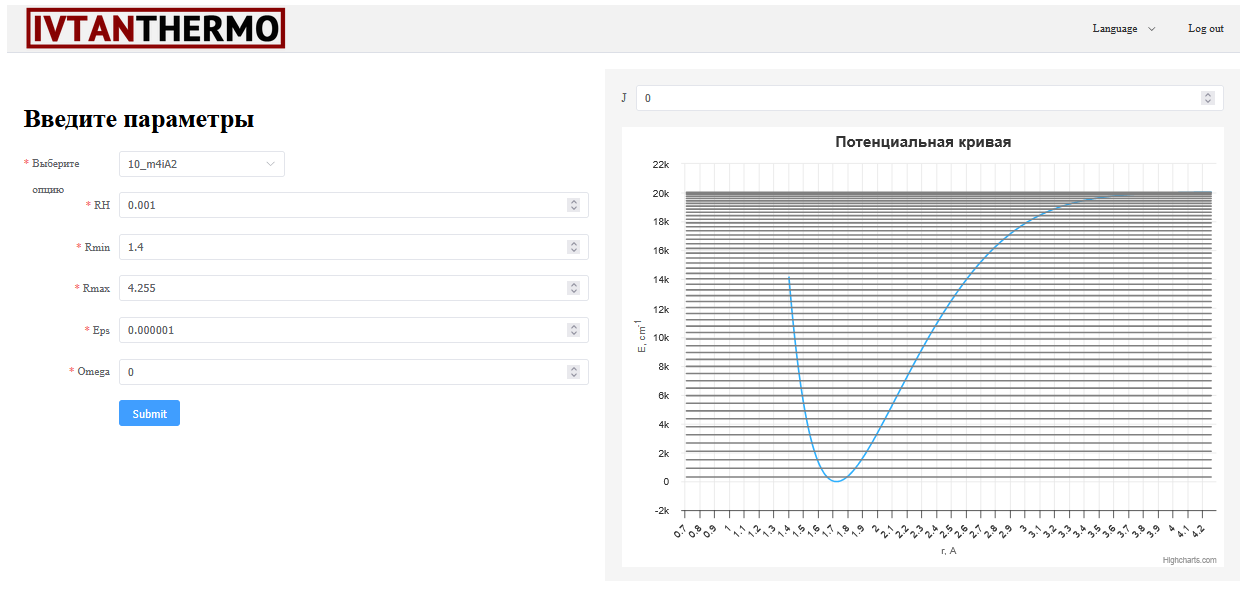
\includegraphics[width=1\linewidth]{images/gasthermo_level}
		\caption{\label{fig:gasthermo_level} Интерфейс веб-приложения GasThermo, программный модуль работы с LEVEL}
	\end{figure}
	
	    \begin{figure}[ht]
		\centering
		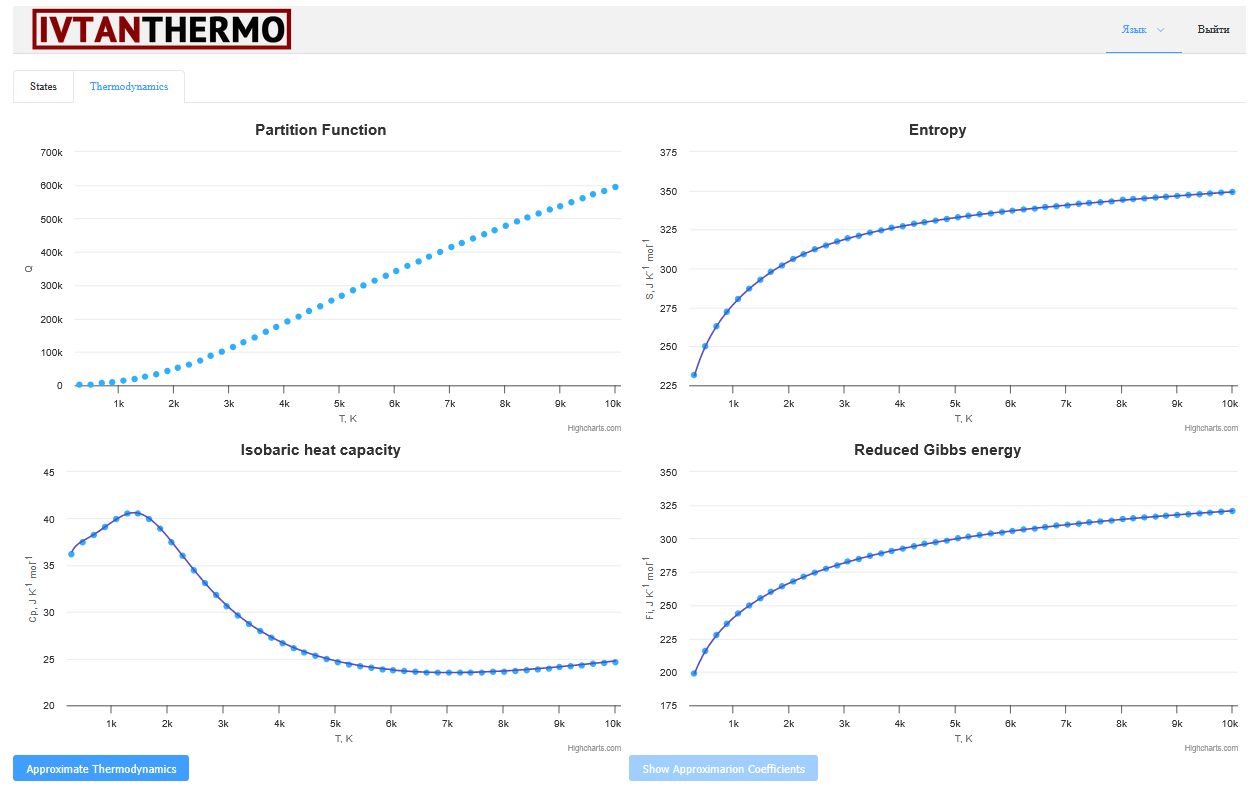
\includegraphics[width=1\linewidth]{images/gasthermo_thermo}
		\caption{\label{fig:gasthermo_thermo} Интерфейс веб-приложения GasThermo, программный модуль работы Partion Function с аппроксимацией}
	\end{figure}
    \newpage
    \section{Расчет термодинамических функций ArC$^+$}
    
    \subsection{Результаты расчетов потенциальных кривых}
    \label{sec:Chapter3.1}
    
    Полученные межатомные потенциалы обоих пределов диссоциации показаны на рисунке \ref{fig:states_all}. Разность энергий между двумя пределами в 4.295 eV и значительная глубина потенциальных ям возбужденных состояний, показанных сплошными кривыми, предполагают заметный вклад последних в термодинамические функции при более высоких температурах. 
    
    Поведение каждого состояния определяется его доминирующей конфигурационной функцией, отражающей определенную орбитальную заселенность. В нескольких случаях имеются две ведущие конфигурации, взаимно симметричные относительно заселенностей орбиталей $p_x$ и $p_y$. Краткий анализ этих функций дает приблизительное представление о причинах возникновения потенциальных ям в рамках отдельных состояний. Отметим, что во всех случаях орбиталь C(2s) является дважды заселенной, а пары орбиталей $p_x$, $p_y$ и $p_z$ Ar и C -- сонаправлены.
    
    Первый предел характеризуется тремя состояниями -- $^2 \Pi_x$, $^2 \Pi_y$ и $^2 \Sigma^+$. Как отмечено в \cite{tuttle}, молекулярное взаимодействие можно сопоставить с притяжением электронного облака аргона ионизированным углеродом. В таком случае электронная плотность занятой орбитали C(2p$_z$) в состоянии $^2 \Sigma^+$ противодействует этому взаимодействию, тогда как заселение орбиталей C(2p$_x$) и C(2p$_y$) в состоянии $^2 \Pi$ ограничивает его слабее, приводя к более выраженной потенциальной яме. Аналогичная интерпретация может быть применена к состояниям второго предела: один отсутствующий электрон уменьшает экранирование заряда ядра аргона. В случаях с однократно занятой орбиталью Ar(3p$_z$) взаимодействие между зарядом ядра аргона и электронной плотностью углерода является наиболее сильным. Поэтому состояния $(1)^4 \Sigma^-$ и $(1)^4 \Pi$ характеризующийся подобной заселенностью имеют наиболее глубокие потенциальные ямы, для $(1)^4 \Sigma^-$ этот эффект дополнительно усиливается пустой орбиталью C(2p$_z$).
    
    Другой вариант заселенности предполагает максимальное число электронов на молекулярных орбиталях $p_z$, с дважды занятой орбиталью Ar(3p$_z$) и одним электроном на C(2p$_z$). Различные перестройки оставшихся электронов формируют множество энергетически близких состояний: по два первых состояния в группах $^2A_1$, $^2A_2$, $^4A_1$ и $^4A_2$, за которыми близко следует оставшееся слабосвязанное состояние $(2)^2\Pi$. В этой нотации первое целое число обозначает номер состояния в рамках данной симметрии, тогда как верхний индекс обозначает спиновую мультиплетность. Каждое из этих состояний имеет мелкую яму приблизительно 800--1000 cm$^{-1}$, они отдельно выделены в дополнительной панели рисунка \ref{fig:states_all}. Совокупное влияние этих состояний на термодинамические функции не позволяет исключить их из обсуждения. В данной работе мы обозначаем их согласно вырожденным или близколежащим парам, которые они образуют в интервале расстояний 2.5--5 \AA, охватывающем область их потенциальных ям: $^4\Delta_1$ и $^4\Delta_2$, образованные парами $A_1/A_2$, а также отдельные близко лежащие пары $^2\Sigma^+/^2\Sigma^+$ и $^2\Sigma^-/^2\Sigma^-$. При дальнейшем уменьшении межатомного расстояния состояния $(1)^2\Delta$ и $(2)^2\Sigma^+$ образуют дополнительные ямы вследствие избегаемых пересечений с состояниями из другого предела диссоциации.
    
    Для лучшей читаемости и понимания причин возникновения потенциальных ям второго предела, описанных ранее, в таблице \ref{tab:configs} представлены ведущие конфигурации (заселенности молекулярных орбиталей) состояний для $R = 3.5$ \AA. В случае соответствия нескольких конфигураций одному состоянию подразумевается их равнозначный вклад в волновую функцию, что также указывает на присутствующее влияние статистической корреляции при определении энергии этих состояний.
    
    \begin{figure}[ht]
    	\centering
    	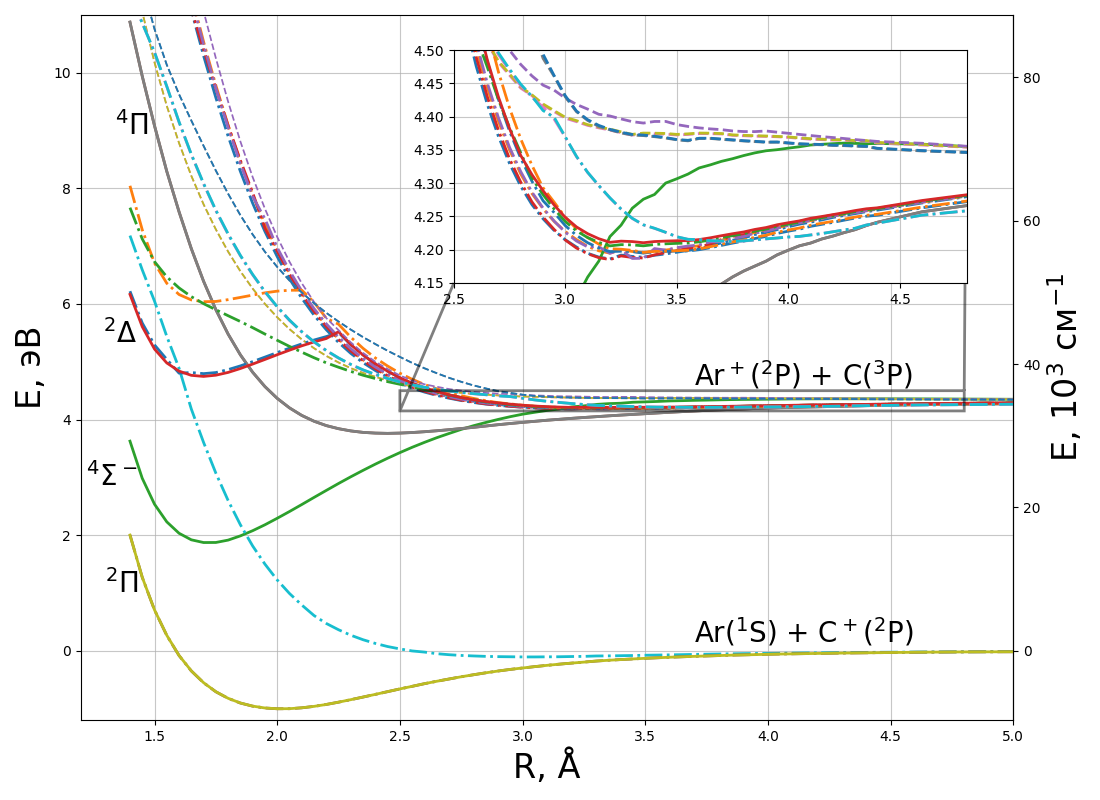
\includegraphics[width=1\linewidth]{images/states_all}
    	\caption{\label{fig:states_all} Кривые межатомных потенциалов ArC$^+$ без спин-орбитального и спин-спинового расщепления.}{Сильно связанные состояния ($D_e > 2000$ см$^{-1}$) показаны сплошными линиями, слабо связанные ($D_e < 2000$ см$^{-1}$)-- штрихпунктирной линией, оттаивающие -- пунктиром. Дополнительная панель показывает слабосвязанные состояния $^2\Pi$, $^4\Delta_1$, $^4\Delta_2$, $^2\Sigma^+/^2\Sigma^+$ и $^2\Sigma^-/^2\Sigma^-$.}
    \end{figure}
    
    \begin{table}[ht]
    	\centering
    	\footnotesize
    	\begin{tabular}{|c|cccccc|c|}
    		\hline
    		Молек. орбиталь            & \multicolumn{1}{c|}{Ar (3p$_\text{x}$)} & \multicolumn{1}{c|}{Ar (3p$_\text{y}$)} & \multicolumn{1}{c|}{Ar (3p$_\text{z}$)} & \multicolumn{1}{c|}{C (2p$_\text{x}$)} & \multicolumn{1}{c|}{C (2p$_\text{y}$)} & C (2p$_\text{z}$) & $D_e$, см$^{-1}$ \\ \hline
    		Предел                     & \multicolumn{6}{c|}{Ar($3s^23p^6$; $^1$S) -- C$^+$($2s^22p^1$; $^2$ P)}                                                                                                                                                           &                  \\ \hline
    		$X^2\Pi_x$                 & 2                                       & 2                                       & 2                                       & 1                                      & 0                                      & 0                 & 8115.5           \\ \cline{1-7}
    		$X^2\Pi_y$                 & 2                                       & 2                                       & 2                                       & 0                                      & 1                                      & 0                 &                  \\ \hline
    		$(1)^2\Sigma^+$            & 2                                       & 2                                       & 2                                       & 0                                      & 0                                      & 1                 & 870.2            \\ \hline
    		Предел                     & \multicolumn{6}{c|}{Ar$^+$($3s^23p^5$; $^2$P) -- C($2s^22p^2$; $^3$P)}                                                                                                                                                            &                  \\ \hline
    		$(1)^4\Sigma^-$            & 2                                       & 2                                       & 1                                       & 1                                      & 1                                      & 0                 & 20063.1          \\ \hline
    		$(1)^4\Pi_x$               & 2                                       & 2                                       & 1                                       & 1                                      & 0                                      & 1                 & 4414.8           \\ \cline{1-7}
    		$(1)^4\Pi_y$               & 2                                       & 2                                       & 1                                       & 0                                      & 1                                      & 1                 &                  \\ \hline
    		$^4D_1 (A_1)$              & 2                                       & 1                                       & 2                                       & 0                                      & 1                                      & 1                 & 1011.5           \\
    		& 1                                       & 2                                       & 2                                       & 1                                      & 0                                      & 1                 &                  \\ \cline{1-7}
    		$^4D_1 (A_2)$              & 2                                       & 1                                       & 2                                       & 1                                      & 0                                      & 1                 &                  \\
    		& 1                                       & 2                                       & 2                                       & 0                                      & 1                                      & 1                 &                  \\ \hline
    		$^4D_2 (A_1)$              & 2                                       & 1                                       & 2                                       & 0                                      & 1                                      & 1                 & 996.0            \\
    		& 1                                       & 2                                       & 2                                       & 1                                      & 0                                      & 1                 &                  \\ \cline{1-7}
    		$^4D_2 (A_2)$              & 2                                       & 1                                       & 2                                       & 1                                      & 0                                      & 1                 &                  \\
    		& 1                                       & 2                                       & 2                                       & 0                                      & 1                                      & 1                 &                  \\ \hline
    		$^2\Sigma^+/^2\Sigma^+$(a) & 2                                       & 1                                       & 2                                       & 0                                      & 1                                      & 1                 & 858.3            \\
    		& 1                                       & 2                                       & 2                                       & 1                                      & 0                                      & 1                 &                  \\ \cline{1-7}
    		$^2\Sigma^+/^2\Sigma^+$(b) & 2                                       & 1                                       & 2                                       & 0                                      & 1                                      & 1                 &                  \\
    		& 1                                       & 2                                       & 2                                       & 1                                      & 0                                      & 1                 &                  \\ \hline
    		$^2\Sigma^-/^2\Sigma^-$(a) & 2                                       & 1                                       & 2                                       & 1                                      & 0                                      & 1                 & 843.0            \\
    		& 1                                       & 2                                       & 2                                       & 0                                      & 1                                      & 1                 &                  \\ \cline{1-7}
    		$^2\Sigma^-/^2\Sigma^-$(b) & 2                                       & 1                                       & 2                                       & 1                                      & 0                                      & 1                 &                  \\
    		& 1                                       & 2                                       & 2                                       & 0                                      & 1                                      & 1                 &                  \\ \hline
    		$(2)^2 \Pi_x$              & 2                                       & 2                                       & 1                                       & 1                                      & 0                                      & 1                 & 702.9            \\ \cline{1-7}
    		$(2)^2 \Pi_y$              & 2                                       & 2                                       & 1                                       & 0                                      & 1                                      & 1                 &                  \\ \hline
    		$(2)^4\Pi_x$               & 2                                       & 1                                       & 2                                       & 1                                      & 1                                      & 0                 & --               \\ \hline
    		$(2)^4\Pi_y$               & 1                                       & 2                                       & 2                                       & 1                                      & 1                                      & 0                 & --               \\ \hline
    		$(3)^2\Pi_x$               & 2                                       & 1                                       & 2                                       & 1                                      & 1                                      & 0                 & --               \\ \hline
    		$(3)^2\Pi_y$               & 1                                       & 2                                       & 2                                       & 1                                      & 1                                      & 0                 & --               \\ \hline
    		$(3)^2\Sigma^-$            & 2                                       & 2                                       & 1                                       & 1                                      & 1                                      & 0                 & --               \\ \hline
    	\end{tabular}
	    \caption{\label{tab:configs} Ведущие конфигурации состояний ArC$^{+}$}
    \end{table}
    
    \subsection{Сравнение с предыдущими работами}
    \label{sec:Chapter3.2}
    
    В этом разделе мы сравниваем полученные результаты с предыдущими теоретическими исследованиями и экспериментальными данными из \cite{hillier}. Спектроскопические постоянные $D_e$ и $r_e$ были получены из EMO-аппроксимации наших потенциальных кривых, а затем использованы совместно с первыми двумя уровнями рассчитанного вращательно-колебательного спектра для получения констант $\omega_e$, $\omega_e x_e$, $B_e$ и $\alpha_e$. Все параметры потенциалов приведены в таблице \ref{tab:spectroscopic}. 
    
    %Для лучшей читаемости таблицы сравнение ограничивается данными, полученными с использованием методов coupled-cluster и configuration-interaction, в то время как полный набор упомянутых в литературном обзоре данных приведен в Приложении \ref{sec:Apendix}.
    
    Для первых трех состояний ArC$^+$ наши результаты показывают хорошее согласие по большинству параметров с потенциалом из \cite{hillier}, который был восстановлен инверсией данных рассеяния. Хотя значение $D_e$ немного выше, оно находится в пределах приведенной экспериментальной неопределенности 10\%. Для потенциалов ab initio подробное сравнение предыдущих результатов было приведено в \cite{tuttle}, также выделяющее общую тенденцию последовательного углубления потенциальных ям при использовании все более продвинутых методов. Сравнение потенциальной кривой основного состояния с двумя упомянутыми источниками приведен на рисунке \ref{fig:compare}. 
    
    Для второго предела диссоциации единственным доступным источником данных, которые мы смогли найти, являются расчеты POL-CI из \cite{hillier} для состояний $(1)^4 \Sigma^-$ и $(1)^4 \Pi$, где использовался сжатый базис 7s5p1d для аргона и базис 5s3p1d для углерода. Как и ожидалось, расчеты на основе семейства базисов aug-cc-pwCVnZ ввиду большего числа молекулярных орбиталей дают более глубокие ямы и отличающиеся спектроскопические постоянные. Также для данного предела нами были впервые получены ППЭ 15-и состояний, из которых $^2\Pi$, $^4\Delta_1$, $^4\Delta_2$, $^2\Sigma^+/^2\Sigma^+$ и $^2\Sigma^-/^2\Sigma^-$ являются слабосвязанными в интервале расстояний 2.5--5 \AA. Состояния $(1)^2\Delta$ и $(2)^2\Sigma^+$ обладают дополнительными ямами в области мылах расстояний, образованными эффектом избегаемого пересечения.
    
    \begin{figure}[ht]
    	\centering
    	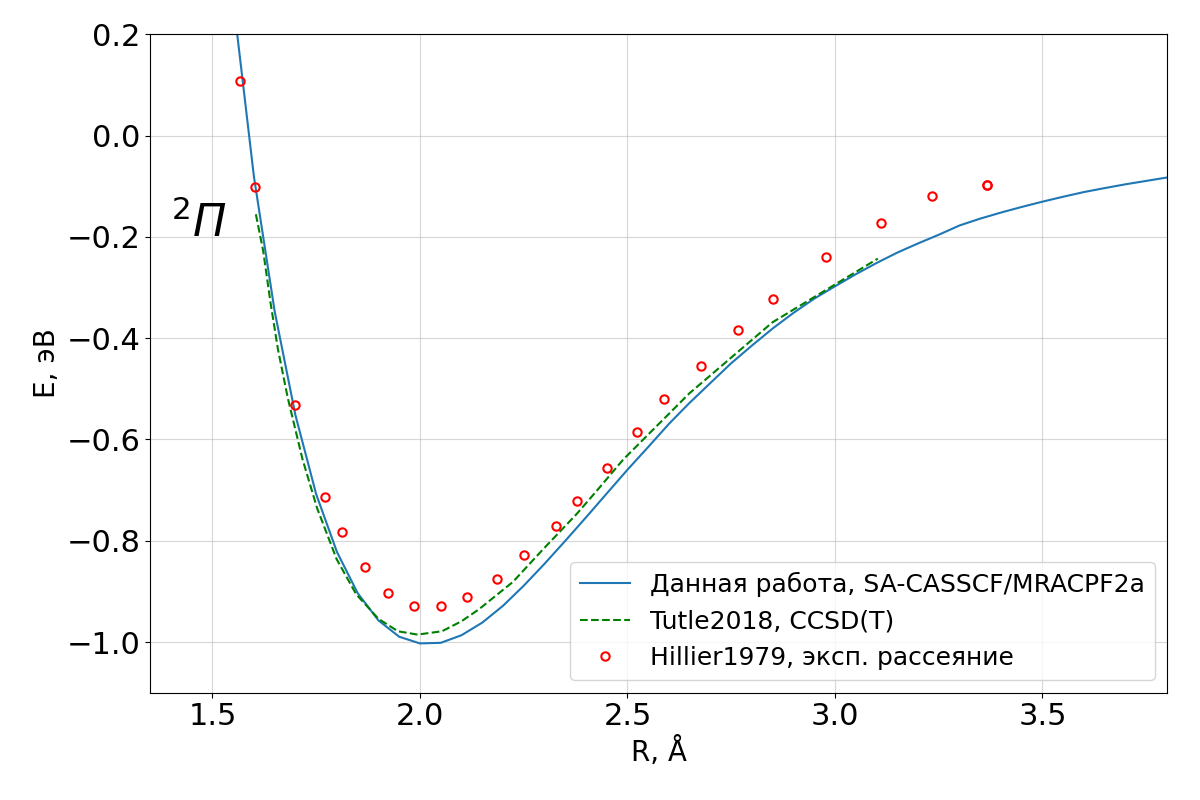
\includegraphics[width=0.9\linewidth]{images/compare}
    	\caption{\label{fig:compare} Сравнение данных о ППЭ основного состояния ArC$^+$}
    \end{figure}
    
    \begin{table}[ht]
    	\centering
    	\footnotesize	
    	\begin{tabular}{|c|c|c|c|c|c|c|c|c|}
    		\hline
    		& $r_e$, \AA & $D_e$, см$^{-1}$ & $T_e$, см$^{-1}$ & $\omega_e$, см$^{-1}$ & $\omega_e x_e$, см$^{-1}$ & $B_e$, см$^{-1}$ & $\alpha_e$, см$^{-1}$ & Источник                     \\ \hline
    		$X^2\Pi$                & 2.017            & 8115.5           & -                & 415.8                 & 5.33                      & 0.449            & 7.11                  & Данная работа                  \\
    		& 1.995            & 7570.0           &                  & 417.0                 & 6.00                      & 0.515            & 9.20                  & \cite{hillier}, Рассеяние   \\
    		& 1.996            & 7982.2           &                  & 413.2                 & 4.17                      & 0.458            & 6.21                  & \cite{tuttle}, RCCSD(T)/$\infty$Z \\
    		& 1.999            & 8024.9           &                  & 413.1                 &                           &                  &                       & \cite{tuttle}, MRCI/QZ       \\
    		& 2.000            & 9520.0           &                  & 485.0                 & 6.50                      & 0.511            & 8.30                  & \cite{hillier}, Pol-CI       \\
    		& 2.004            & 8100.0           &                  &                       &                           &                  &                       & \cite{froudakis}, CCSD(T)/DZ \\ \hline
    		$(1)^2\Sigma^+$         & 3.030            & 870.2            & 7232.8           & 125.0                 & 4.49                      & 0.199            & 7.12                  & Данная работа                  \\
    		& 2.997            & 1006.2           &                  & 120.9                 &                           &                  &                       & \cite{tuttle}, MRCI          \\
    		& 3.009            & 901.5            &                  & 115.8                 &                           &                  &                       & \cite{tuttle}, RCCSD(T)/$\infty$Z      \\ \hline
    		$(1)^4\Sigma^-$         & 1.721            & 20063.1          & 23196.4          & 730.8                 & 6.65                      & 0.617            & 7.13                  & Данная работа                  \\
    		& 1.762            & 16502.8          &                  & 777.00                & 9.10                      & 0.644            & 8.80                  & \cite{hillier}, Pol-CI       \\ \hline
    		$(1)^4\Pi$              & 2.443            & 4414.8           & 38430.1          & 296.9                 & 4.99                      & 0.306            & 5.75                  & Данная работа                  \\
    		& 2.548            & 2855.2           &                  & 234                   & 5.00                      & 0.315            & 7.60                  & \cite{hillier}, Pol-CI       \\ \hline
    		$^4D_1$                 & 3.200            & 1011.5           & 41846.3          & 120.9                 & 3.61                      & 0.178            & 5.53                  & Данная работа                  \\
    		$^4D_2$                 & 3.326            & 996.0            & 41859.9          & 125.7                 & 3.96                      & 0.165            & 5.08                  & Данная работа                  \\
    		$^2\Sigma^+/^2\Sigma^+$ & 3.350            & 858.3            & 41924.5          & 89.5                  & 2.33                      & 0.163            & 4.95                  & Данная работа                  \\
    		$^2\Sigma^-/^2\Sigma^-$ & 3.350            & 843.0            & 42012.5          & 88.2                  & 2.31                      & 0.163            & 4.98                  & Данная работа                  \\
    		$(2)^2 \Pi$             & 3.734            & 702.9            & 42065.0          & 79.4                  & 2.24                      & 0.131            & 4.07                  & Данная работа                  \\
    		$(1)^2\Delta$           & 1.701            & 6242.1           & 46375.7          & 709.2                 & 20.14                     & 0.631            & 15.67                 & Данная работа                  \\
    		$(2)^2\Sigma^+$         & 1.711            & 1604.9           & 56806.1          & 753.5                 & 88.45                     & 0.624            & 33.81                 & Данная работа                  \\ \hline
    	\end{tabular}
    	
    	\caption{\label{tab:spectroscopic} Спектроскопические постоянные потенциалов ArC$^{+}$}
    \end{table}
    
    
    \subsection{Термодинамические функции}
    \label{sec:Chapter3.3}
    
    Для расчета термодинамических функций использовались кривые потенциальной энергии всех связанных состояний, их энергетические спектры были объединены для получения итоговых результатов, представленных сплошными линиями на рисунке \ref{fig:thermo}. Табличные данные для всех термодинамических потенциалов в температурном диапазоне 298.15 -- 20000 K представлены в \ref{tab:thermo_points}, а их полиномиальная аппроксимация \ref{eq:ivtan_polynom} приведена в таблице \ref{tab:thermo_polynom}.
    
    Стоит подчеркнуть важность включения энергетических уровней возбужденных состояний в температурную зависимость статистической суммы при высоких температурах. На рисунке \ref{fig:thermo} дополнительно изображены кривые термодинамических функций, нанесенные пунктирными линиями. Самая нижняя кривая соответствует случаю, в котором рассматривается только основное состояние, тогда как каждая следующая по высоте кривая включает в расчет статистической суммы энергетические уровни дополнительного возбужденного состояния. Соответственно самая высокая (сплошная) кривая соответствует включению всех рассмотренных связанных состояний. 
    
    Рассмотрим зависимость относительного отклонения $\varepsilon\{X\}$ первой пунктирной кривой (учет только основного состояния) от сплошной (учет всех состояний) на графике термодинамической функции $X$. В таблице \ref{tab:epsilons} даны значения данного отклонения для $X \in \{ C_p^\circ,\ \Delta H^\circ,\ \Phi^\circ,\ S^\circ\}$ в основных температурных точках. Стоит отметить разницу в порядках между погрешностями для разных термодинамических функций, показывающую особую чувствительность $C_p^\circ$ и $\Delta H^\circ$ к учету возбужденных состояний.
    
    \begin{table}[ht]
    	\centering
    	\begin{tabular}{|c|c|c|c|c|}
    		\hline
    		T, K     & $\varepsilon\{C_p\}$, \%    & $\varepsilon\{\Delta H\}$, \% & $\varepsilon\{ \Phi \}$, \% & $\varepsilon\{S\}$, \%    \\ \hline
    		5000  & 0.61  & 0.61   & 0.08 & 0.14 \\
    		10000 & 14.83 & 3.12   & 0.16 & 0.41 \\
    		15000 & 26.49 & 9.12   & 0.36 & 1.04 \\
    		20000 & 27.66 & 13.76  & 0.62 & 1.62 \\ \hline
    	\end{tabular}
 	    \caption{\label{tab:epsilons} Относительное отклонение $\varepsilon\{X\}$ для $X \in \{ C_p^\circ,\ \Delta H^\circ,\ \Phi^\circ,\ S^\circ\}$}
    \end{table}
    
    Особенно заметное влияние можно увидеть в случае изобарной теплоемкости $C_\text{p}$, где ситуация усугубляется в сравнении с постоянно возрастающими в абсолютном значении термодинамическими функциями. На рисунке \ref{fig:relative_thermo} вынесены зависимости $\varepsilon\{C_p\}$ для кривых с последовательным увеличением набора учитываемых состояний. По полученным зависимостям $\varepsilon \{ C_\text{p} \} $(T) видно, что при температурах выше 4000 K возбужденные состояния второго предела начинают играть существенную роль в корректном описании термодинамических потенциалов. При рассмотрении области температур до 10000 K, характерной для условий масс спектрометрии с индуктивно связанной плазмой (ИСП-МС), можно выделить следующие особенности:
    
    \begin{enumerate}
    	\item Для точного описания первого локального максимума теплоемкости (до 3000 К) необходимо включение основного и первого возбужденного состояния.
    	
    	\item Описание теплоемкости в области температур ИСП-МС с погрешностью не выше 7\% требует включения первых 4-х состояний.
    	
    	\item Для точного описания теплоемкости на всем промежутке температур ИСП-МС (погрешность менее 1\%) обязательно включение связанных состояний обоих пределов (первые 16 состояний).
    \end{enumerate}
    
    \begin{figure}[ht]
    	\centering
    	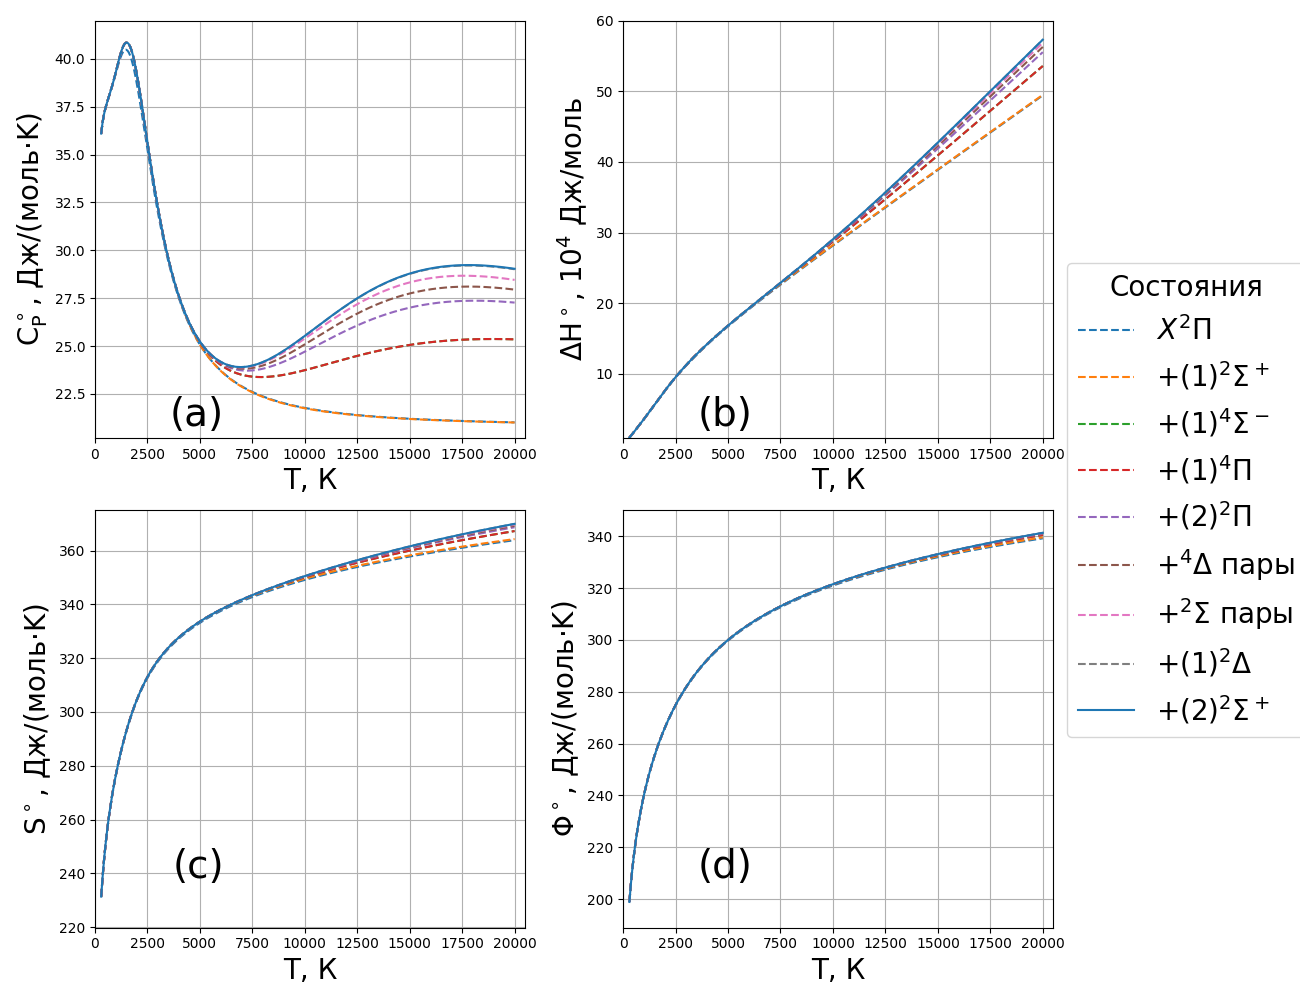
\includegraphics[width=1\linewidth]{images/thermo}
    	\caption{\label{fig:thermo} Термодинамические функции ArC$^+$ при 298.15 -- 20000 K}{Пунктирные линии представляют температурные зависимости, рассчитанные с различным числом учитываемых состояний, каждая из которых подписана последним состоянием, добавленным в набор. Самая нижняя пунктирная линия соответствует использованию только основного состояния, тогда как самая верхняя сплошная соответствует включению всех связанных состояний, доступных из расчетов SA-CASSCF/MRACPF2a.}
    \end{figure}
    \begin{figure}[ht]
    	\centering
    	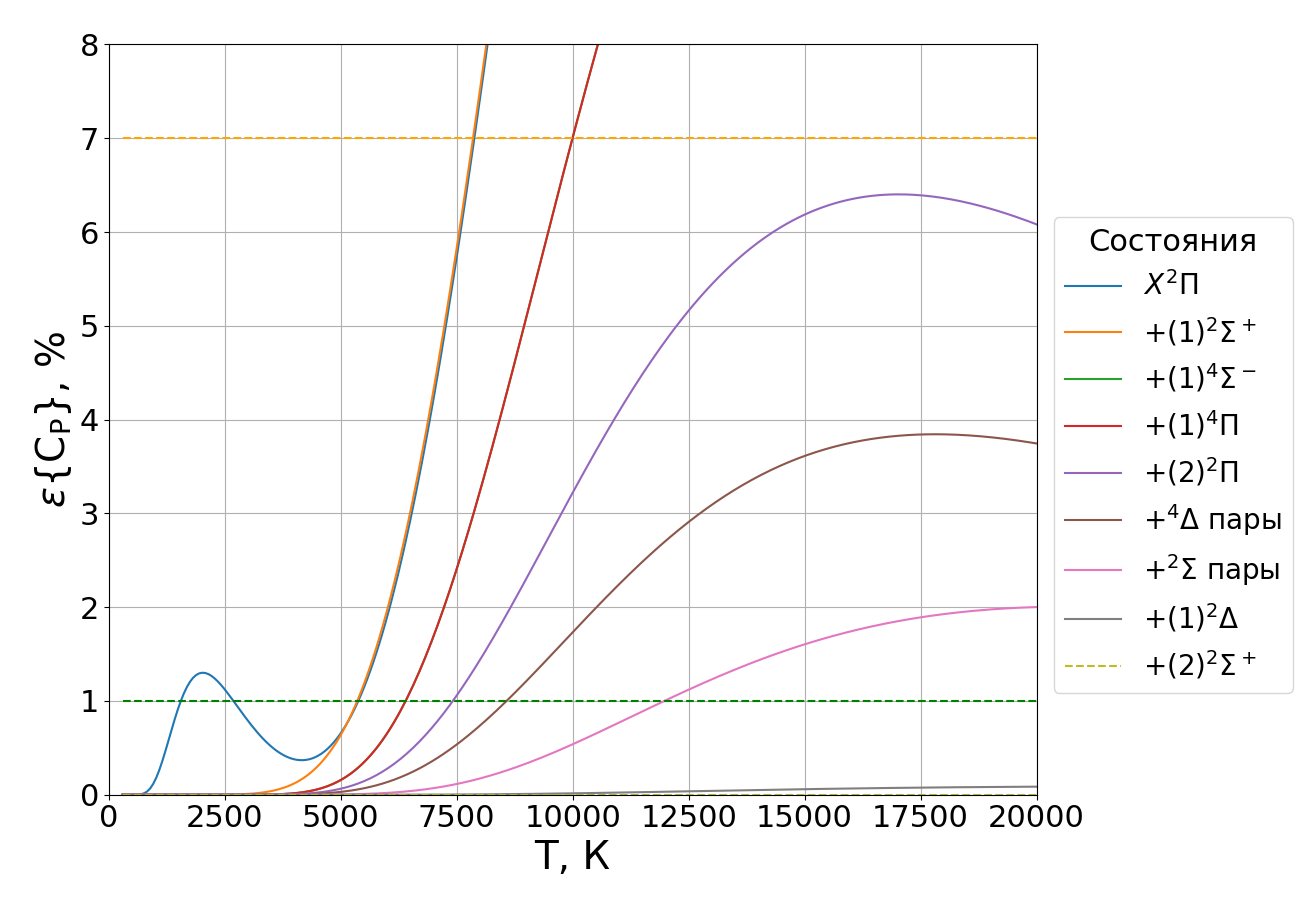
\includegraphics[width=1\linewidth]{images/compare_thermo}
    	\caption{\label{fig:relative_thermo} Относительное отклонение изобарной теплоемкости с неполным учетом состояний от случая, учитывающего все связанные состояния ArC$^+$}
    \end{figure}
    
    \begin{table}[ht]
    	\small
    	\centering
    	\begin{tabular}{|c|c|c|c|c|}
    		\hline
    		T, K  & $C_{\mathrm{P}}^\circ$, J/(mol·K) & ${\mathrm{\Phi}}^\circ$, J/(mol·K) & $\mathrm{S}^\circ$, J/(mol·K) & ${\mathrm{\Delta H}}^\circ$, $10^4$ J/mol \\ \hline
    		300   & 36.10                      & 198.8                       & 231.3                                        & 0.98                                \\
    		400   & 36.91                      & 208.3                       & 241.8                                        & 1.34                                \\
    		500   & 37.41                      & 215.9                       & 250.1                                        & 1.71                                \\
    		600   & 37.79                      & 222.2                       & 257.0                                        & 2.09                                \\
    		700   & 38.14                      & 227.6                       & 262.8                                        & 2.47                                \\
    		800   & 38.49                      & 232.3                       & 268.0                                        & 2.85                                \\
    		900   & 38.88                      & 236.6                       & 272.6                                        & 3.24                                \\
    		1000  & 39.31                      & 240.4                       & 276.7                                        & 3.63                                \\
    		1200  & 40.18                      & 247.1                       & 284.0                                        & 4.42                                \\
    		1400  & 40.77                      & 252.8                       & 290.2                                        & 5.24                                \\
    		1600  & 40.80                      & 257.8                       & 295.7                                        & 6.05                                \\
    		1800  & 40.24                      & 262.3                       & 300.4                                        & 6.86                                \\
    		2000  & 39.20                      & 266.3                       & 304.6                                        & 7.66                                \\
    		3000  & 32.31                      & 281.7                       & 319.2                                        & 11.24                               \\
    		4000  & 27.62                      & 292.2                       & 327.7                                        & 14.20                               \\
    		5000  & 25.25                      & 299.9                       & 333.6                                        & 16.82                               \\
    		6000  & 24.17                      & 305.9                       & 338.1                                        & 19.29                               \\
    		7000  & 23.90                      & 310.8                       & 341.8                                        & 21.69                               \\
    		7500  & 23.98                      & 312.9                       & 343.4                                        & 22.88                               \\
    		8000  & 24.16                      & 314.9                       & 345.0                                        & 24.09                               \\
    		9000  & 24.75                      & 318.4                       & 347.9                                        & 26.53                               \\
    		10000 & 25.52                      & 321.5                       & 350.5                                        & 29.04                               \\
    		11000 & 26.35                      & 324.2                       & 353.0                                        & 31.64                               \\
    		12000 & 27.13                      & 326.7                       & 355.3                                        & 34.31                               \\
    		13000 & 27.83                      & 329.0                       & 357.5                                        & 37.06                               \\
    		14000 & 28.38                      & 331.2                       & 359.6                                        & 39.87                               \\
    		15000 & 28.79                      & 333.1                       & 361.6                                        & 42.73                               \\
    		16000 & 29.06                      & 335.0                       & 363.5                                        & 45.63                               \\
    		17000 & 29.20                      & 336.7                       & 365.2                                        & 48.54                               \\
    		18000 & 29.23                      & 338.3                       & 366.9                                        & 51.46                               \\
    		19000 & 29.15                      & 339.9                       & 368.5                                        & 54.36                               \\
    		20000 & 29.01                      & 341.3                       & 370.0                                        & 57.26                              \\ \hline
    	\end{tabular}
    	\caption{\label{tab:thermo_points} Термодинамические функции ArC$^{+}$ для температурного диапазона 298.15 -- 20000 K}{}
    \end{table}
    
    \begin{table}[ht]
    	\begin{tabular}{|c|c|c|c|c|c|c|c|}
    		\hline
    		T, K               & $\phi_1$ & $\phi_2$ & $\phi_3$ & $\phi_4$ & $\phi_5$ & $\phi_6$ & $\phi_7$  \\ \hline
    		300.0 -- 827.1     & 319.45   & 35.98    & -0.0005  & 0.1617   & 29.46    & -104.79  & 323.9026  \\
    		827.1 -- 1354.2    & 360.76   & 50.11    & -0.0045  & 0.6896   & -158.41  & 516.41   & -767.5688 \\
    		1354.2 -- 2078.9   & 164.26   & -32.49   & 0.0652   & -4.6618  & 481.38   & -725.81  & 521.5462  \\
    		2078.9 -- 3133.1   & 449.69   & 117.27   & -0.2616  & 10.9288  & -242.73  & 155.19   & -53.6117  \\
    		3133.1 -- 4582.6   & 386.72   & 72.23    & 0.0037   & 3.1831   & -112.42  & 61.40    & -17.8078  \\
    		4582.6 -- 8404.0   & 342.02   & 34.45    & 0.3507   & -4.9029  & -23.98   & 9.57     & -1.5889   \\
    		8404.0 -- 12093.6  & 330.88   & 7.65     & 1.4813   & -17.2258 & 5.07     & 1.73     & -0.4673   \\
    		12093.6 -- 18155.2 & 322.27   & -33.53   & 4.1216   & -40.5415 & 41.45    & -6.31    & 0.4799    \\
    		18155.2 -- 20000.0 & 311.46   & 16.17    & -3.4308  & 2.6726   & 12.73    & -2.14    & 0.1570    \\ \hline
    	\end{tabular}
    	\caption{\label{tab:thermo_polynom} Полиномиальные коэффициенты для аппроксимации термодинамических функций ArC$^{+}$ в температурном диапазоне 298.15 -- 20000 K}{}
    \end{table}
    
    
    \newpage
    \section{Расчет термодинамических функций ArC}
    
    \subsection{Результаты расчета и сравнение потенциальных кривых}
    \label{sec:Chapter4.1}
	
	Для молекулы ArC были получены состояния 6-ти различных пределов, на рисунке \ref{fig:states_all2} изображены лишь связанные, а также по одному состоянию на оставшиеся пределы. В данном случае все состояния легко различимы, что позволяет привести набор точных термов на каждом пределе вместе со значением энергии предела на уровне диссоциации относительно уровня диссоциации основного состояния:
	
	\begin{enumerate}
		\item $\text{Ar}\left({ }^1 S_g\right)\text{ -- }\text{C}\left({ }^3 P_g ; 2 s^2 2 p^2\right)$: ${ }^3 \Sigma^{-},{ }^3 \Pi$; 
		\item $\operatorname{Ar}\left({ }^1 S_g\right) \text{ -- }\text{C}\left({ }^1 D_g ; 2 s^2 2 p^2\right)$: ${ }^1 \Sigma^{+},{ }^1 \Pi,{ }^1 \Delta$
		\item $\operatorname{Ar}\left({ }^1 S_g\right) \text{ -- } \text{C}\left({ }^1 S_g ; 2 s^2 2 p^2\right)$: ${ }^1 \Sigma^{+}$
		\item $\operatorname{Ar}\left({ }^1 S_g\right) \text{ -- } \text{C}\left({ }^5 S_u ; 2 s^1 2 p^3\right)$: ${ }^5 \Sigma^{-}$
		\item $\operatorname{Ar}\left({ }^1 S_g\right) \text{ -- } \text{C}\left({ }^3 P_u ; 2 s^2 2 p^1 3 s^1\right)$: ${ }^3 \Sigma^{+},{ }^3 \Pi$
		\item $\operatorname{Ar}\left({ }^1 S_g\right) \text{ -- } \text{C}\left({ }^3 D_u ; 2 s^1 2 p^3\right)$: ${ }^3 \Sigma^{-},{ }^3 \Pi,{ }^3 \Delta$
	\end{enumerate}
	
	Среди них только высоколежащие состояния $(2)^3\Pi$ и $(3)^3\Pi$ являются связанными, в то время как основное состояние $X^3\Sigma^-$ обладает малозначительной ямой в 101.9 см$^{-1}$. При этом состояния группы $^3\Pi$ участвуют во взаимных квазипересечениях, из-за чего дополнительно уменьшается глубина ямы $(3)^3\Pi$. Для описания данных функций использовался EMO-потенциал с высоким значением $N_\beta$ для сглаживания ППЭ, такой выбор оправдан резкостью квазипересечения из-за отсутствия в расчетах спин-орбитального взаимодействия. Полученные данные спектроскопических констант приведены в таблице \ref{tab:spectroscopic2}.
	
	Из рассмотренной литературы удалось найти единичный ab initio расчет \cite{Sohlberg}, затрагивающий ППЭ Ван дер Вальсовой молекулы ArC на уровне MRCI. Представленные результаты для связанного состояния $(2)^3\Pi$ также сравниваются в таблице \ref{tab:spectroscopic2}, данные текущей работы лежат хорошем согласии по основным спектроскопическим константам. Дополнительно в таблице \ref{tab:limits2} приведено сравнение уровней энергии диссоциации между данной работой и доступными в \cite{Sohlberg} результатами.
	
	
	\begin{table}[h!]
		\centering
		\begin{tabular}{|c|c|c|c|c|}
			\hline
			& $r_e$, \AA & $D_e$, см$^{-1}$ & $w_e$, см$^{-1}$ & Источник       \\ \hline
			$X^3\Sigma^-$ & 3.230 & 101.9  & 176.3 & Эта работа     \\ \hline
			$(2)^3\Pi$      & 1.914 & 4665.4 & 190.7 & Эта работа     \\ \cline{2-5} 
			& 1.955 & 5079.1 & 225.6 & {[}Sohlberg{]} \\ \hline
			$(3)^3\Pi$      & 1.748 & 8118.4 & 190.7 & Эта работа     \\ \hline
		\end{tabular}
		\caption{Спектроскопические константы связывающих состояний ArC}
		\label{tab:potentials2}
	\end{table}
    
    \subsection{Термодинамические функции}
    \label{sec:Chapter4.2}
    
    По кривым потенциальной энергии были также рассчитаны термодинамические функции ArC (см [РИС 4]), данные о температурной зависимости и интервальном полиномиальном описании приведены в Таблицах \ref{tab:thermo2} и \ref{tab:polynoms2}.
    
    
    \begin{table}[h!]
    	\centering
    	\begin{tabular}{|c|c|c|c|c|}
    		\hline
    		T, K & C$_{\mathrm{P}}$, Дж/(моль·K) & ${\mathrm{\Phi}}$, Дж/(моль·K) & ${\mathrm{S}}$, Дж/(моль·K) & ${\mathrm{\Delta H}}$, $10^4$ Дж/моль \\ \hline
    		300  & 21.09                         & 198.2                          & 221.8                       & 0.71                                  \\ \hline
    		400  & 20.96                         & 204.9                          & 227.9                       & 0.92                                  \\ \hline
    		500  & 20.89                         & 210.0                          & 232.6                       & 1.13                                  \\ \hline
    		600  & 20.86                         & 214.1                          & 236.4                       & 1.34                                  \\ \hline
    		700  & 20.84                         & 217.5                          & 239.6                       & 1.55                                  \\ \hline
    		800  & 20.83                         & 220.4                          & 242.4                       & 1.75                                  \\ \hline
    		900  & 20.82                         & 223.0                          & 244.8                       & 1.96                                  \\ \hline
    		1000 & 20.81                         & 225.3                          & 247.0                       & 2.17                                  \\ \hline
    		1200 & 20.80                         & 229.2                          & 250.8                       & 2.59                                  \\ \hline
    		1400 & 20.80                         & 232.5                          & 254.0                       & 3.00                                  \\ \hline
    		1600 & 20.80                         & 235.4                          & 256.8                       & 3.42                                  \\ \hline
    		1800 & 20.79                         & 237.9                          & 259.2                       & 3.84                                  \\ \hline
    		2000 & 20.79                         & 240.2                          & 261.4                       & 4.25                                  \\ \hline
    		3000 & 20.79                         & 248.7                          & 269.8                       & 6.33                                  \\ \hline
    		4000 & 20.79                         & 254.8                          & 275.8                       & 8.41                                  \\ \hline
    		5000 & 20.81                         & 259.5                          & 280.5                       & 10.49                                 \\ \hline
    		6000 & 21.22                         & 263.4                          & 284.4                       & 12.62                                 \\ \hline
    		7000 & 22.71                         & 266.6                          & 287.7                       & 14.75                                 \\ \hline
    		7500 & 24.71                         & 268.1                          & 289.3                       & 15.93                                 \\ \hline
    		8000 & 28.02                         & 269.5                          & 291.0                       & 17.25                                 \\ \hline
    		8500 & 31.89                         & 271.4                          & 292.9                       & 18.26                                 \\ \hline
    		9000 & 38.71                         & 272.6                          & 294.9                       & 20.01                                 \\ \hline
    		9500 & 47.56                         & 273.9                          & 297.2                       & 22.16                                 \\ \hline
    		9999 & 59.58                         & 275.3                          & 300.7                       & 25.39                                 \\ \hline
    	\end{tabular}
    	\caption{Температурная зависимость термодинамических функций ArC}
    	\label{tab:thermo2}
    \end{table}
    
    \begin{table}[h!]
    	\centering
    	\begin{tabular}{|c|c|c|c|c|c|c|c|}
    		\hline
    		Интервал T, K     & $\phi_1$  & $\phi_2$  & $\phi_3$  & $\phi_4$  & $\phi_5$   & $\phi_6$  & $\phi_7$  \\ \hline
    		300.0 - 3594.3    & 274.141  & 20.791   & 0.000    & -0.095   & -0.029    & 0.039    & -0.025   \\ \hline
    		3594.31- 5307.3   & 257.295  & 7.213    & 0.111    & -2.835   & 33.625    & -20.839  & 6.897    \\ \hline
    		5307.4 - 6954.5   & 61.041   & -200.033 & 3.172    & -59.048  & 417.232   & -199.115 & 51.281   \\ \hline
    		6954.5 - 8404     & 229.085  & 80.880   & -4.986   & 48.337   & 52.636    & -81.940  & 31.438   \\ \hline
    		8404.0 - 9655.8   & 1876.447 & 3376.260 & -123.344 & 1444.024 & -3842.296 & 1070.322 & -150.585 \\ \hline
    		9655.85 - 10000.0 & 2723.213 & 5390.381 & -207.539 & 2366.014 & -6037.289 & 1667.147 & -236.978 \\ \hline
    	\end{tabular}
    	\caption{Полиномиальное описание термодинамических функций ArC}
    	\label{tab:polynoms2}
    \end{table}
    
    \newpage
    \section{Заключение}
    \label{sec:Chapter5}
    
    Межатомные потенциалы для двух пределов диссоциации были рассчитаны на уровне теории CASSCF/MRACPF2a. Спектроскопические постоянные, полученные для состояний $X^2 \Pi$ и $(1)^2 \Sigma^+$, хорошо согласуются с доступными теоретическими и экспериментальными результатами. Это указывает на то, что вновь полученные кривые для $(1)^2 \Delta$ и $(2)^2\Sigma^+$, а также потенциальные ямы $^2\Sigma^+/^2\Sigma^+$, $^2\Sigma^-/^2\Sigma^-$, $^4\Delta_1$ и $^4\Delta_2$, определенные в диапазоне от 2.5 до 5 \AA, были получены с аналогичной точностью.
    
    С использованием этих данных были получены термодинамические функции для интервала 298.15 -- 20000 K. Сравнение температурных зависимостей, рассчитанных с различным числом включенных состояний, указывает на значительное влияние высоковозбужденных состояний на результаты, особенно при более высоких температурах, типичных для масс-спектрометрии с ICP. Следовательно, точное определение термодинамических функций в температурном диапазоне 5000 -- 6500 K требует включения спектров энергетических уровней по крайней мере четырех низколежащих состояний, тогда как расчеты при 6500 K и выше требуют всех 21 состояний двух пределов диссоциации ArC$^+$.
    
    %% в зависимости от надобности подключаем раздел "Приложение"
    % \newpage
    \section*{Приложение}
    \addcontentsline{toc}{section}{Приложение}
    \label{sec:Apendix}
    
    Здесь необходимо написать приложение, которое вы должны придумать самостоятельно.
    
    \newpage
    %% НЕ ТРОГАЙТЕ!!!
    \nocite{*}
    \bibliography{article}
    
\end{document}
